\documentclass{school-22.211-notes}
\date{March 14, 2012}

\begin{document}
\maketitle

%%%%%%%%%%%%%%%%%%%%%%%%%%%% Exam 1 Review Begin %%%%%%%%%%%%%%%%%%%%%%%%%%%%%%%%%%%%%%%%%%
\lecture{Exam 1 Review: Spectral Calculation}
\topic{Basics}
\begin{enumerate}
\item Know 1.0 kT correspond to 0.0253 eV. Know $\displaystyle u = \ln \frac{E_{\mathrm{ref}}}{E}$. 

\item Know number density $\displaystyle N = \frac{\rho N_A}{M}$, where $N_A$ is  avogado's number, take $0.6022$, $\rho$ is density in g/cc, $M$ is atomic mass (unitless). 

\item In an elastic scattering
  \eqn{ \alpha = \frac{E_{\mathrm{min}}}{E_0} = \left( \frac{A-1}{A+1} \right)^2 < 1 }

\item Mean log energy decrement. Know maximum $\xi$ is $1$ for hydrogen. $A \up, \xi \down$. 
  \eqn{ \xi = 1 + \frac{\alpha \ln \alpha}{1-\alpha} }

\item Number of collisions to slow neutrons from $E_i \to E_f$: $\displaystyle n = \frac{ \ln (E_i/E_f)}{\xi}$. 

\item Moderating power = $\frac{\xi \sigma_s}{\sigma_a}$, a measurement of the slowing down ability. 

\item Flux disadvantage factor (HW4) $\displaystyle = \frac{\phi^M}{\phi^F}$, and thermal group has $>1$, fast group has $<1$. 

\item Spectrum summary:
  \begin{enumerate}
  \item $E < 1$ eV (thermal range): a hardened Maxwellian distribution (hardened because the temperature equilibrium has not been perfectly achieved) plus a 1/E correction at higher energies, $\phi(E) = \phi_M (E, T_n) + \frac{ \lambda \Delta (E/kT_n) }{E}$. 

  \item $1 \eV < E < 50$ keV (slowing-down domain): $\phi(E) \sim \frac{1}{\xi(E) \Sigma_t(E) E}$. 

  \item $E > 0.5$ MeV: $\phi(E) = \frac{\chi(E)}{\Sigma_t(E)}$.
  \end{enumerate}

\item Spectrum peaks:   
  \begin{enumerate}
  \item A hump in high energy. Reason: fission spectrum, degraded due to scattering; 
  \item A slight decrease in the epithermal region. Reason: resonant capture losses, esp. U238; 
  \item A hump in low energy. Reason: Maxwell distribution of the thermal agitation but a little harder because the temperature equilibrium has not been perfectly achieved. 
  \end{enumerate}
\end{enumerate}


\clearpage
\topic{Elastic Scattering Cross Section} 
\begin{enumerate}
\item Elastic Scattering
  \begin{enumerate}
  \item Asymptotic elastic scattering for high energy (above 4eV): assume isotropic scattering in COM. Generate $1/E$ spectrum; asymptotic flux value is $\Phi_{as} (u) = \frac{S}{\xi \Sigma_s (u)}$ according to Reuss (7.2.3). 
  \item Thermal elastic scattering (below 4eV): use elastic scattering for monatomic (Maxwellian) free gas; may up-scatter. 
  \end{enumerate}

\item Lab system: $\theta$ is uniformly distributed, front favored. 
  \eqn{ \frac{E_f}{E_i} = \frac{1}{2} \left[ 1 + \alpha + (1-\alpha) \cos \theta \right] } 

\item CMCS: $\cos \theta$ is uniformly distributed, that is, elastic scattering is isotropic in CMCS. 
  \eqn{ P(E_i \to E_f) &= \frac{1}{(1-\alpha) E_i}  &  E_f &\in [\alpha E_i, E_i] }
  \eqn{ \sigma_s (E_i \to E_f) = \sigma_s (E_i) P(E_i \to E_f) }
  \begin{figure}[ht]
    \centering
    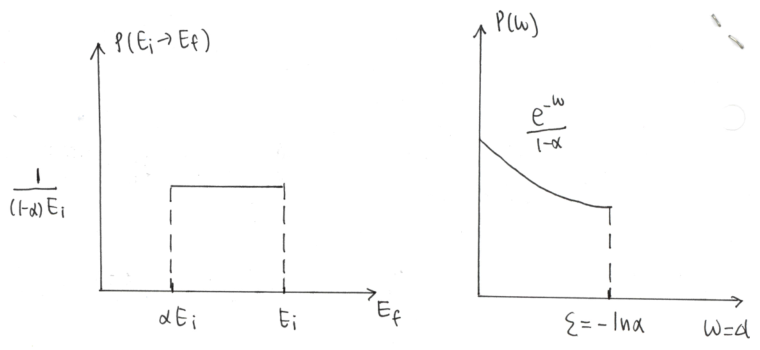
\includegraphics[width=4in]{images/sl-d/prob.png}
  \end{figure}


  This concept was tested multiple times:
  \begin{itemize}
    \item  \textbf{12 Qual \#1c}: what's the probability of neutrons slowing down from 1 MeV to 100 keV from elastically scattering off Hydrogen? 

      Answer: recall hydrogen has a flat distribution, so $P = \frac{100 \mathrm{keV}}{1 \MeV} = 10\%$. 
    \item \textbf{12 Exam 1 \#11}: what's the probability that a neutron scattering off a hydrogen atom at 10 eV will have its next collision within the energy interval of Absorbium's $E_0$ = 6.67 eV resonance? 

      Answer: Absorbium's resonance is from 6.17eV to 7.17eV. That's asking starting from 10eV what's the chance of falling in between 6.17eV and 7.17eV. Answer is 10\%. 

    \item \textbf{12 Exam 1 \#12}: what's the probability that a neutron scattering off a hydrogen atom at 200 eV will have its next collision within the energy interval of Absorbium's $E_0$ = 57.3 eV resonance? 

      Answer: the exact same thing as the last problem, we get $P = \frac{1 \eV}{200 \eV} = 0.0005$. 
  \end{itemize}

\end{enumerate}


\clearpage
\topic{Slowing Down Equation to Solve For Spectrum} 
\begin{enumerate}
\item Slowing down equation (omitting the $E$ dependency): 
  \eqn{ \Sigma_t \phi = \int_0^{\infty} \Sigma_s (E' \to E) \phi (E') + \chi (E) S_f} 
  
\item Fast range: sl-d equation simplifies to, 
  \eqn{ \Sigma_t \phi &= \chi S_f   & \phi(E) &= \frac{\chi(E) S_f}{\Sigma_t} }
  
\item Intermediate range: we define a slowing down density/current, 
  \eqn{ q(E) = \mbox{\# neutrons cross energy $E$ per time per volume} }
  sl-d equation simplifies to, 
  \eqn{ \frac{\dq (E)}{\dE} = - \Sigma_a (E) \phi (E) }
  For regions that we can assume $\Sigma_a = 0$ (e.g., between resonances), 
  \eqn{ q(E) &= \mbox{constant},  & \phi(E) &= \frac{q(E)}{\xi \Sigma_s (E) E} }

\item Thermal range: assume thermal equilibrium, pure scattering xs, infinite medium, we get a Maxwellian spectrum. See next section for more details.
\end{enumerate}

\clearpage
\topic{Doppler Effect on Cross Sections}
We only discuss thermal range for now. Resonance range is reserved for next time. 
\begin{enumerate}
\item Basic: Maxwellian spectrum $+$ stationary target $+$ free target. We get $\sigma_s$ depends on $A, E, T$. Using free gas model, now upscattering is possible. This is where we implemented those erf() functions and get plots like, 
  \begin{figure}[ht]
  \centering
  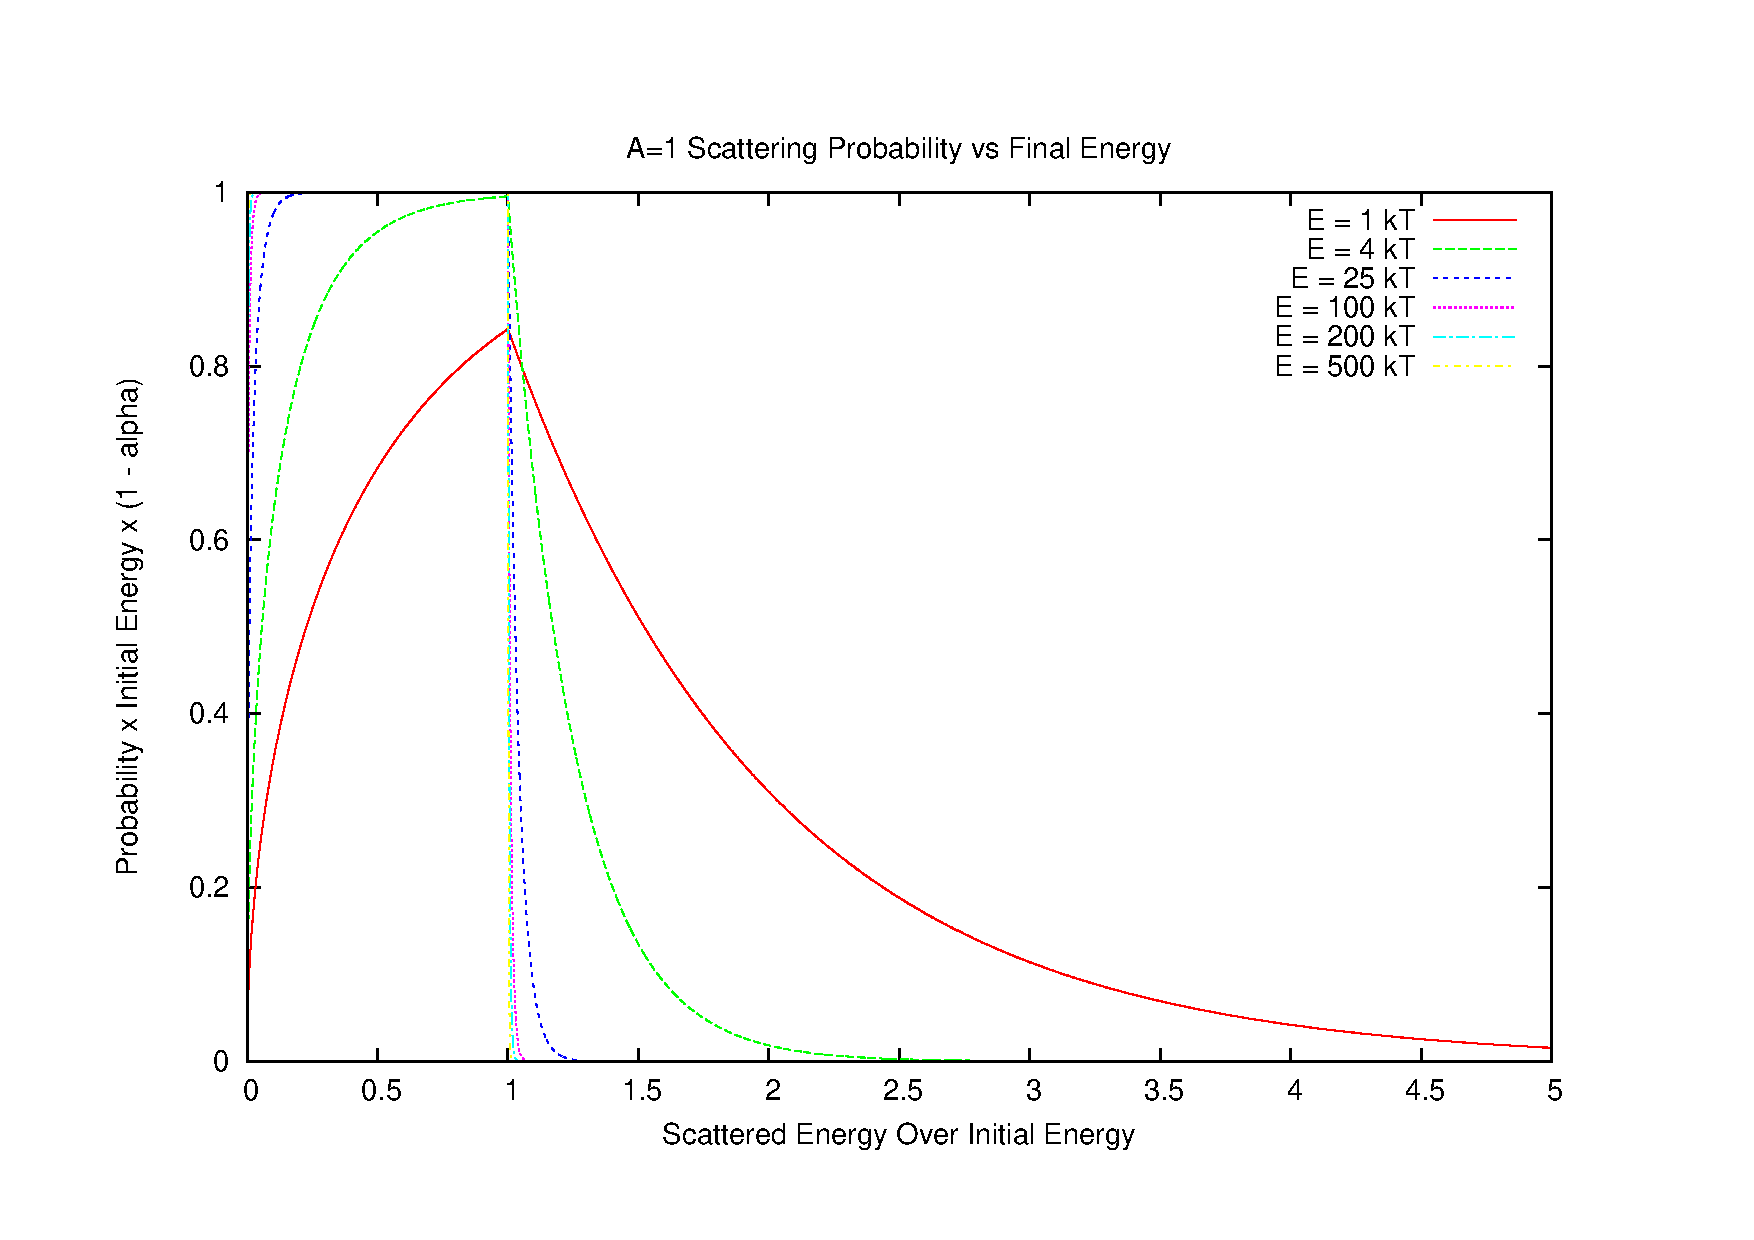
\includegraphics[width=3in]{images/sl-d/ts_H.uncrop.pdf}
  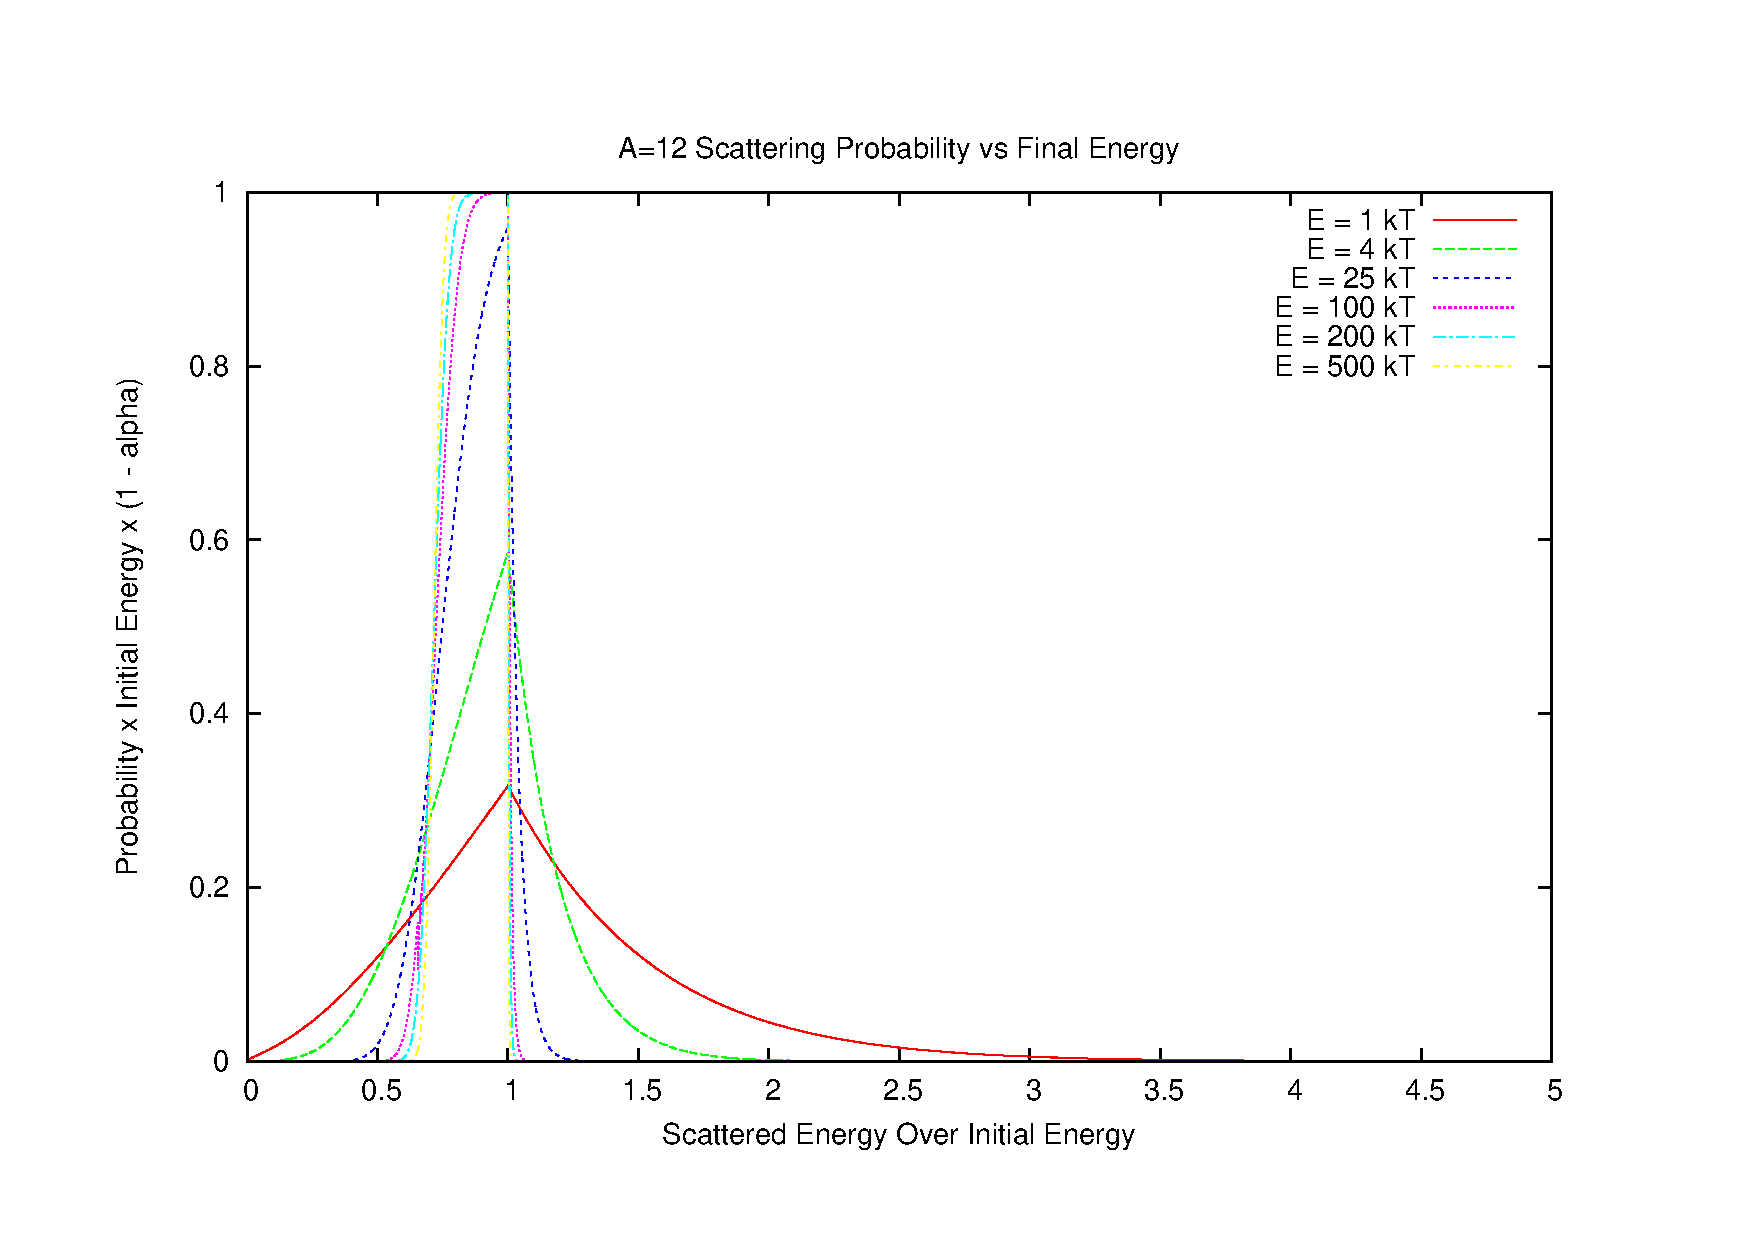
\includegraphics[width=3in]{images/sl-d/ts_C.uncrop.pdf}
\end{figure}
 
\textbf{12 Exam 1 \# 8}: we are given a pdf symmetric about $E'/E = 1$. What's the probability that a 0.0253 eV neutron would be scattered to a higher energy in a collision with this thermal gas at 293K? 

Answer: 0.5, because of the symmetry. 

\textbf{12 Exam 1 \# 9}: the cdf of this kernel predicts a probability of 0.0333 for a 0.025 eV neutron to be scattered to energies greater than 0.05 eV in a material at 300K. If one uses the same curve to model the gas at 1200K, what would be the probability that 0.10 eV neutrons would be scattered above 0.20 eV in the same gas at 1200K? 

Answer: 0.0333. The ratio is all it matters. 

\textbf{12 Exam 1 \# 10}: draw and label the scattering kernel that you would predict for $kT = 20$. 

Answer: the plot is probability vs. $E_{out}/E_{in}$, and it should be a box. 

\item Add target motion/Doppler temperature effects: 
\begin{figure}[ht]
  \centering
  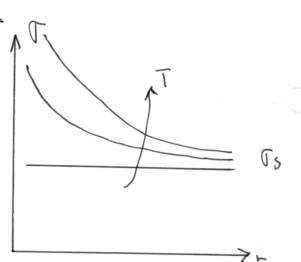
\includegraphics[width=1.6in]{images/sl-d/Doppler.png}
\end{figure}
\textbf{12 Exam 1 \#4,5}: If the neutron cross section is independent of energy at a temperature of 0K, what energy shape do you expect for the neutron xs at 1200K? Why? 

Answer: $1/v$ shape, thermal motion/vibration.

\item Add chemical bond. $\displaystyle \sigma_{\mathrm{bound}} = \left( \frac{A+1}{A} \right)^2 \sigma_{\mathrm{free}}$.   Know the $S(\alpha, \beta)$ term. 
\end{enumerate}

\clearpage
\topic{Resonances and Doppler} 
\begin{enumerate}
\item SLBW Model for cross sections: the SLBW scattering cross section is, 
  \eqn{ \sigma_s (x) &= \frac{2}{\Gamma} (r \psi(x) + q \chi(x)) + \sigma_p}
  where 
  \eqn{ x &= \frac{2(E -E_0)}{\Gamma} &\psi &= \frac{1}{1+x^2} &\chi&= \frac{2x}{1+x^2} }
  \textbf{Spring 2012 Exam 1 \#6:} given $r,q, \Gamma,T$, at what energy does the scattering cross section peak? 
  \begin{itemize}
  \item Solve for $\frac{\dsigma_s}{\dx} = 0$ for $x$, then plug into the definition for $x$ for $E$.
  \item Alternatively, in this problem $r \ll q$, $\chi$ dominate the scattering cross section, and $\chi$ maximize at $x=1$, hence $x=1$. 
  \end{itemize}

\item Doppler effects
  \begin{enumerate}
    \item Psi/chi functions

      \begin{figure}[ht]
        \centering
        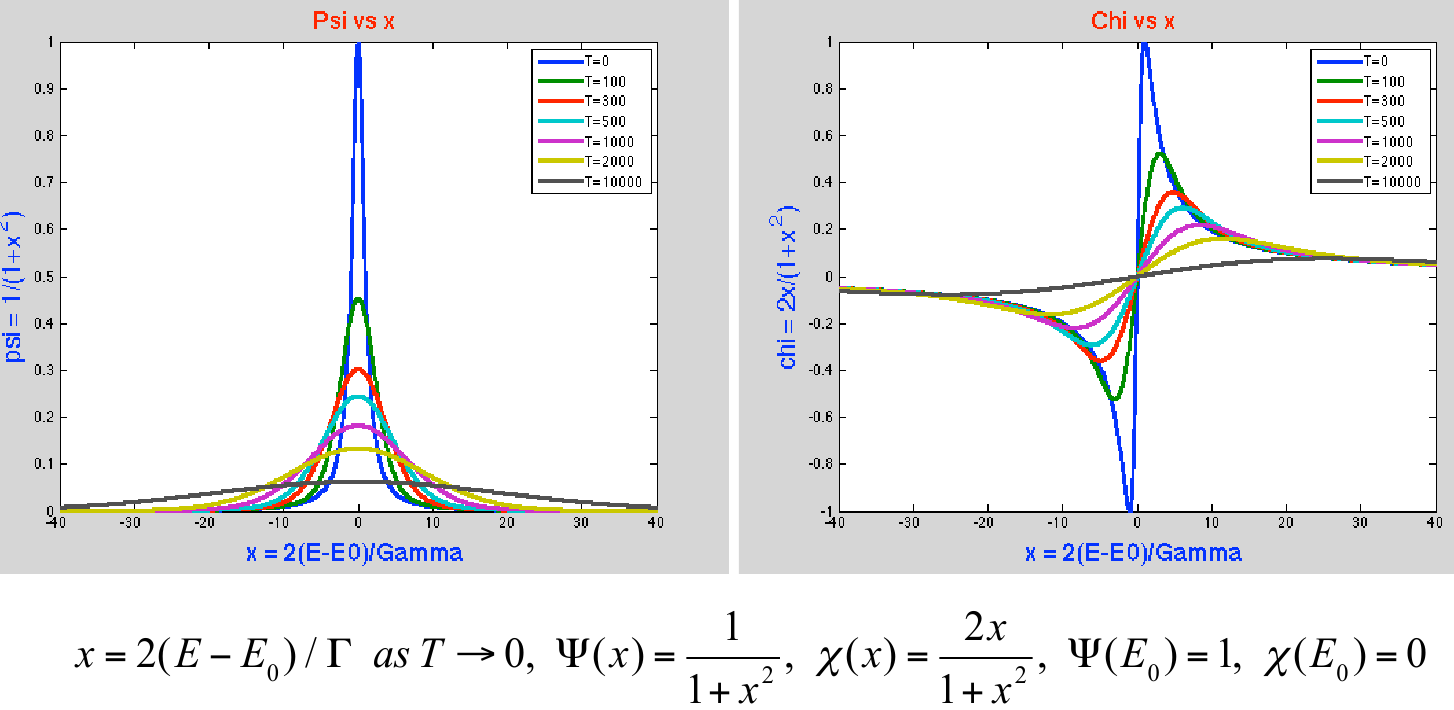
\includegraphics[width=6in]{images/r-m/psi-chi-plot.png}
      \end{figure}

    \item Finite dilution: $\boxed{U/H \down, \RIeff \down}$ because of energy self-shielding: as U/H increases, more and more self-shielding, the flux is more depressed, result in smaller $\RIeff$. A second consequence is that the higher energy range becomes more important. See Section~\ref{spectral-hardening-section}. 
    \item Temperature effects: $\boxed{T \up, \RIeff \up}$ becasue the broadened resonance increases the energy range over which abosprtion occurs. There is less flux depression, whereas the area under the cross section is about the same, result in an increase in the $\RIeff$. 

\textbf{Spring 2012 Exam 1 \#16:} What is the value of the 300K infinite dilute RI for absorbium integrated from 0 to 20 keV? (we calculated in the previous problem the RI for 0K.)

Answer: \hi{the infinite dilute RI is independent of temperature because in Doppler broadening the area under the resonance is constant.}
  \end{enumerate}
\end{enumerate}

\clearpage
\topic{Homogeneous Resonance Self-sheilding}
  \begin{enumerate}
    \item Infinite media: In infinite medium, the flux shape near resonance depends only on the ratio of the number density of the moderator to the resonance absorber and the moderator cross section. The absolute numbers are not needed until we move into a finite medium and start to worry about leakage. 

    \item Know how to calculate group cross sections. \textbf{2012 Spring Exam 1, \#14}: what is the value of the Absorbium infinite dilute microscopic absorption cross section (in barns) integrated from 100 eV to 20 keV? Answer: 
      \eqn{ \Aboxed{ \expect{\sigma} &= \frac{\int_{E_1}^{E_2} \sigma(E) \phi(E) \dE}{\int_{E_1}^{E_2} \phi(E) \dE} = \frac{\int_{E_1}^{E_2} \sigma(E) \frac{1}{E} \dE}{\int_{E_1}^{E_2} \frac{1}{E}  \dE} = \frac{RI}{\ln\left(\frac{E_2}{E_1} \right)} } }
      Infinite dilute implies that here is no neutrons being absorbed by the resonances. Recall that in HW2 when our U/H is small, the flux is not perturbed by U238 resonances at all, suggesting that the resonance escape probability is one.

    \item Dilution factors/dilution cross section/background cross section, where $r$ is resonance material, $m$ is moderator, $ \displaystyle \boxed{\sigma_d = \frac{N_m \sigma_m}{N_r} }$. 

    \item Resonance Integral
      \begin{enumerate}
      \item Calculation, \textbf{2012 Spring Exam 1, \#13,\#15}, notice $\sigma$ is given independent of E for simplicity,
        \eqn{ \boxed{ \RIeff = - \int_{u1}^{u2} \sigma(u) \du = \int_{E_1}^{E_2} \sigma(E) \frac{1}{E} \dE = \sigma \ln \left( \frac{E_2}{E_1} \right) } }
        where $\sigma$ is the resonance xs, not including potential xs. If there are multiple resonances, sum them up with flux-weighting. 

      \item RI represents the average absorption xs characterizing the resonance, averaged over the flux within the resonance. It conserves the reaction rate/collision density. 
        
      \item Relating to $\sigma_g, \sigma_d$: 
        \eqn{ \RIeff &= \sigma_g \ln \left(\frac{E_2}{E_1} \right)  & \RIeff^{u1\to u2} &= \int_{u1}^{u2} \sigma_a^R (u) \frac{\sigma_d}{\sigma_a^R(u) + \sigma_d} \du  }

      \item Narrow resonance $\RIeff$ approximation: assume any scattering with the resonant material scatters neutrons below the resonance energy. 
        \textbf{Spring 2012 Exam 1 \#18}, assuming $1/E$ spectrum, homogeneous mixture of a scattering material and a resonance absorpting material. 
        \eqn{ \RI_{NR} = \int_{E_1}^{E_2} \sigma_r (E) \frac{\sigma_{pr} + \sigma_d}{\sigma_r(E) + \sigma_{pr} + \sigma_d} \frac{1}{E} \dE = \sigma_r \frac{\sigma_{pr} + \sigma_d}{\sigma_r + \sigma_{pr} + \sigma_d} \ln \left(\frac{E_2}{E_1} \right) }        
        
      \item Wide resonance $\RIeff$ approximation: assume scattering with the resonance material leaves the neutron within the resonance energy and they will be absorbed. \textbf{Spring 2012 Exam 1 \#19}.
        \eqn{ \RI_{WR} = \int_{E_1}^{E_2} \sigma_r (E) \frac{\sigma_d}{\sigma_r(E) + \sigma_d} \frac{1}{E} \dE = \sigma_r \frac{ \sigma_d}{\sigma_r +  \sigma_d} \ln \left(\frac{E_2}{E_1} \right) }  
      \end{enumerate}
  \end{enumerate}

\clearpage
\topic{Heterogeneous Self-Shielding} 
  \begin{enumerate}
    \item Homogeneous/heterogeneous equivalence: 
      \begin{align*}
        \mbox{Homogeneous mixture energy shape of flux } \phi(u) &= \frac{\sigma_{pot, f} + \sigma_d}{\sigma_{r,f} (u) + \sigma_{pot, f} + \sigma_d}   & \sigma_d &= \frac{N_m \sigma_m}{N_r}  \\
       \Aboxed{ \mbox{Heterogeneous energy shape of flux in the fuel } \phi_f(u) &= \frac{\sigma_{pot, f} + \sigma_e}{\sigma_{r,f} (u) + \sigma_{pot, f} + \sigma_e}}   & \Aboxed{ \sigma_e &= \frac{S_f}{4 V_f N_r}  }
      \end{align*}

    \item Escape probabilities $p$: only depends on effective RI and dilution xs: 
      \eqn{ p \approx \exp \left( - \frac{\RI_{\eff}}{\zeta \sigma_d} \right) = \exp \left( - \frac{N_r \RI_{\eff}}{\zeta \Sigma_m} \right)  }
      Escape cross section $\sigma_e$:      $ \sigma_e = \frac{1}{l N_f} = \frac{S}{4V N_f}$. 

      \textbf{Spring 2012 Exam 1 \#17:} what is the resonance escape probability for infinitely dilute material 1 in 1 gm/cc material 2? 
 
      Answer: Material 1 is infinitely dilute, so we assume the flux is shaped entirely by material 2 and hence is not affected by the resonances. $p = 1$. 
 
    \item 2-region reciprocity relation: $\displaystyle \boxed{ P_{1\to 2} \Sigma_1 V_1 = P_{2\to 1} \Sigma_2 V_2}$. 

    \item Collision probability: the most basic form is, 
      \eqn{ P_{ff} = \frac{\sigma_{t,f}(u)}{\sigma_e + \sigma_{t,f}(u)} }

    \item Bell's refinement of the Wigner's rational models, where $b$ depends on geometry and material (opacity) as plotted in Fig.~\ref{bell}.
      \eqn{ P_{ff} = \frac{\sigma_{t,f}(u)}{b \sigma_e + \sigma_{t,f}(u) } }     
      and with Dancoff correction factor, 
      \eqn{ P_{f\to f}  = \frac{\sigma_{t,f} (u)}{\frac{(1-C)b}{(1-C) + Cb} \sigma_e + \sigma_{t,f} (u)}  } 
      where escape cross section is calculated for a cylinder to be $\Sigma_e = \frac{1}{2r}$.  Upon getting $P_{ff}$, we find $P_{fm} = 1 - P_{ff}$, then use reciprocity to find $P_{mf}$. See \textbf{Spring 2012 Exam 1: \#20}. 

    \item Dancoff factors: ratio of probability of next collision happens in a different rod over probability of next collision in any rod. See Fig.~\ref{dancoff} for plot. 
      \begin{itemize}
      \item If the moderator is opaque, the Dancoff factor becomes zero; if transparent, the Danoff factor trends to 1.0. 
      \item $r \up, C \down$. 
      \item $P/D \up C \down$. 
      \end{itemize}

    \item Solving for spatially averaged energy shape of flux in the fuel\footnote{not on the official review sheet} from the first collision rate balance equation.  We construct a first collision rate balance equation (next collision for neutrons in fuel from slowing down source and uncollided flux): 
      \eqn{ N_f \sigma_{t,f} \phi_f V_f = Q_f V_f P_{ff} + Q_m V_m P_{mf} }
      where $Q$ is the slowing down source, and it is assumed to arise from the $1/E$ constant lethargy flux above the resonance energy, 
      \eqn{ Q_m &= N_m \sigma_{s,m} \Phi &Q_f &= N_f \sigma_{pot, f} \Phi }
      Substuiting and dividing by $\Phi$, we get an expression of the fine structure energy shape of flux $f_f = \phi_f / \Phi$, 
      \eqn{ N_f \sigma_{t,f} f_f V_f = N_f \sigma_{pot,f} V_f P_{ff} + N_m \sigma_{s,m} V_m P_{mf} }
      Using reciprocity relation and plug in $P_{ff} = \frac{\sigma_{t.f}}{\sigma_{t,f} + \sigma_e}$, we get the \uline{heterogeneous energy shape} of flux in the fuel: 
      \eqn{ f_f(u) = \frac{\sigma_{pot,f} + \sigma_e}{\sigma_{r,f}(u) + \sigma_{pot,f} + \sigma_e} }
     Comparing with the narrow resonance expression for the homogeneous mixture's energy shape of flux, we notice the only difference the two $\sigma_e$ are replaced by $\sigma_d$. 
  \end{enumerate}



\clearpage
\topic{Other Concepts}
\begin{enumerate}




\item Monte Carlo
  \begin{enumerate}
    \item Physical process:  see Table~\ref{plot-MC}
    \item Collision estimators: \textbf{Spring 2012 Exam 1 \#22:}  \ce{U^{238}} absorption  rate per atom, absorption rate is, respectively, 
      \eqn{ &\Sum \frac{\sigma_a^{238}}{\Sigma_t} & N^{238} \Sum \frac{\sigma_a^{238}}{\Sigma_t} & }
    \item Simple statistics:  need enough to provide resolution, but not too many that each bin does not get enough particles.
  \end{enumerate}
  
\item Pin-cell code: 
  \begin{enumerate}
    \item Flux disadvantage factors: $\frac{\psi^M}{\psi^F}$. 
    \item Fine structure effects. 
    \item Scattering kernel: for larger than 4eV, asymptotic down scattering. For less than 4eV, thermal scattering, approximaetd by elastic scattering for Monatomic/Maxwellian free gas. 
    \item Data: 
      \begin{itemize}
        \item Source from fission spectrum: chi, Maxwell spectrum.
        \item $\sigma_s^H$: read in.
        \item $\sigma_a^H$: $1/v$ absorber.
        \item $\sigma_s^U$: resonance scattering cross section using $\psi, \chi$. 
      \end{itemize}
  \end{enumerate}

\item $1/v$ absorption cross section: 
  \begin{itemize}
  \item Wave-particle duality suggests that slow neutrons see a larger portion of space than fast neutrons, which means that slow neutrons often have larger cross sections, which leads to the 1/v rule for absorption (Reuss, 2.4.1). 
  \item Reason: Breit-Wigner states that absorption cross section is ($i = \gamma$ for radiative capture and $f$ for fission etc):
    \eqn{ \sigma_i = \pi \bar{\lambda}^2 g \frac{\Gamma_n \Gamma_i}{(E - E_0)^2 + \Gamma^2/4}  }
    \begin{itemize}
    \item $\Gamma_f, \Gamma_{\gamma}, \Gamma_{\alpha}$ etc are independent to energy E; $\Gamma_n \sim \sqrt{E}$ (for s-wave);
    \item $\bar{\lambda}^2 \sim \frac{1}{E}$;
    \item The denominator is approximately equal to the constant $E_0^2$ assuming that $E, \Gamma$ are small compared to $E_0$.
    \end{itemize}
    Thus $\sigma_f, \sigma_c \sim \frac{1}{\sqrt{E}} \sim \frac{1}{v}$. Even if several resonances make a contribution, the reasoning remains valid. This reasoning is not valid if $E_0$ is close to zero. 
  \item Henry (p. 202) has a derivation for why $\sigma_a(E_r) \approx \frac{1}{v_r}$, but it is using Breit-Wigner for resonance xs. 
  \end{itemize}
  \textbf{Spring 2012 Exam 1:} if the neutron cross section is independent of energy (flat) at a temperature of 0K, what energy shape would you expect for the neutron cross section at 1200K? why? 
  \begin{itemize}
    \item $\sigma(E) \propto 1/v$.
    \item Phenomenon: neutron energy is on the same order as the thermal vibration of the interaction material. 
  \end{itemize}


\item $1/E$ fluxes: true except when resonant absorber is present (recall we keep using 1/E for spectrum above the resonance). 
  \begin{itemize}
  \item It is characteristic of the scalar flux in the slowing down energy range, as long as there is no up-scattering and no fission source. 
  \item It arises basically from the kinematics of the scattering interaction (asymptotic elastic scattering, more specifically). However it gets distorted by the energy behavior of the scattering cross sections and by neutron-absorption processes (Henry, p. 90). 
  \item Stacy (p.103) derives from slowing-down equation that, with Hydorgen as the only moderator, and very heavy nuclei with $\alpha_j = \left(\frac{A-1}{A+1} \right)^2$:
    \begin{align}
      \Sigma_t(E) \Phi(E) &= \int_E^{\infty} \Sigma_s^H \Phi(E')\frac{\dE'}{E'} + \Sum_{j\neq H} \int_E^{E/\alpha_j} \frac{\Sigma_s^j (E') \Phi(E')}{E'(1-\alpha_j)} \dE' \\
      &=  \int_E^{\infty} \Sigma_s^H \Phi(E')\frac{\dE'}{E'} + \Sum_{j\neq H} \frac{1}{\alpha_j} \Sigma_s^j (E) \Phi(E) \\
      \left[ \Sigma_a (E) + \Sigma_s^H \right] \Phi(E) &= \int_E^{\infty} \Sigma_s^H \frac{\Phi(E')}{E'} \dE' \\
      \phi(E) &= \frac{(\Sigma_a (E_1) + \Sigma_s^H) E_1 \Phi (E_1) }{(\Sigma_a(E) + \Sigma_s^H) E} \exp \left[ - \int_E^{E_1} \frac{\Sigma_a (E') \dE'}{(\Sigma_a(E') + \Sigma_s^H) E'} \right]
    \end{align} 
    suggesting that the neutron energy distribution varies with energy as $\Phi(E) \sim \frac{1}{(\Sigma_a(E) + \Sigma_s^H) E}$. 
  \end{itemize}



\item Maxwellian shapes.
  \begin{itemize}
  \item Fission emission spectrum: peak occurs at 1.7 MeV, average occurs at 2 MeV.
  \item Thermal flux spectrum: for an infintie source-free medium with small absorption cross section (as long as $\Sigma_a(E)$ is small compare to $\Sigma_s(E)$), the thermal spectrum is Maxwellian. The higher energy portion of the thermal region is approximately 1/E with slowing down source and absorption present (Henry, p.98). Stacy (p. 109) provides a more detailed reasoning for why neutron energy distribution in the thermal range can be approximately by Maxwellian distribution: the neutron balance equation in the thermal energy range is, 
    \eqn{ \Sigma_t(E) \phi(E) = \int_0^{E_{th}} \Sigma_s (E' \to E) \phi(E') \dE' + S(E) }
    For the thermal range, we assume no absorption $\Sigma_a(E)$ and no slowing-down source $S(E)$, and we extend the upper limit on the integral to infinity under the assumption that the scattering to energies greater than $E_{th}$ is zero; then the neutron flux balance is,
    \eqn{ \Sigma_s (E) \phi(E) = \int_0^{\infty} \Sigma_s (E' \to E) \phi(E') \dE' }
   It can be shown that a Maxwellian distribution satisfies the above equation. However, absorption, leakage and a slowing-down source would distort the actual spectrum from a Maxwellian. Since most absorption xs vary as 1/v, absorption preferentially removes lower-energy neutrons, effectively shifting the spectrum to higher energies than a Maxwellian at the moderator temperature T. 
  \end{itemize}
  
\item Group cross sections: the contribution of the resonance to a flux-weighted multigroup cross section for reaction type $\gamma$:
  \eqn{ \sigma_{\gamma}^g = \frac{\int_{E_g}^{E_{g-1}} \sigma_{\gamma} (E) \phi(E) \dE}{\int_{E_g}^{E_{g-1}} \phi(E) \dE}  }
  Assume $\phi \sim \frac{1}{E}$,
  \eqn{ \sigma_g = \frac{\RI_{\eff}}{\ln(E_2/E_1)} = \frac{\Sum_{i \in g} RI_i }{\ln{\frac{E_{g-1}}{E_g} }}   }
 

\end{enumerate}

\begin{table}
  \centering
  \begin{tabular}[h]{cl}
    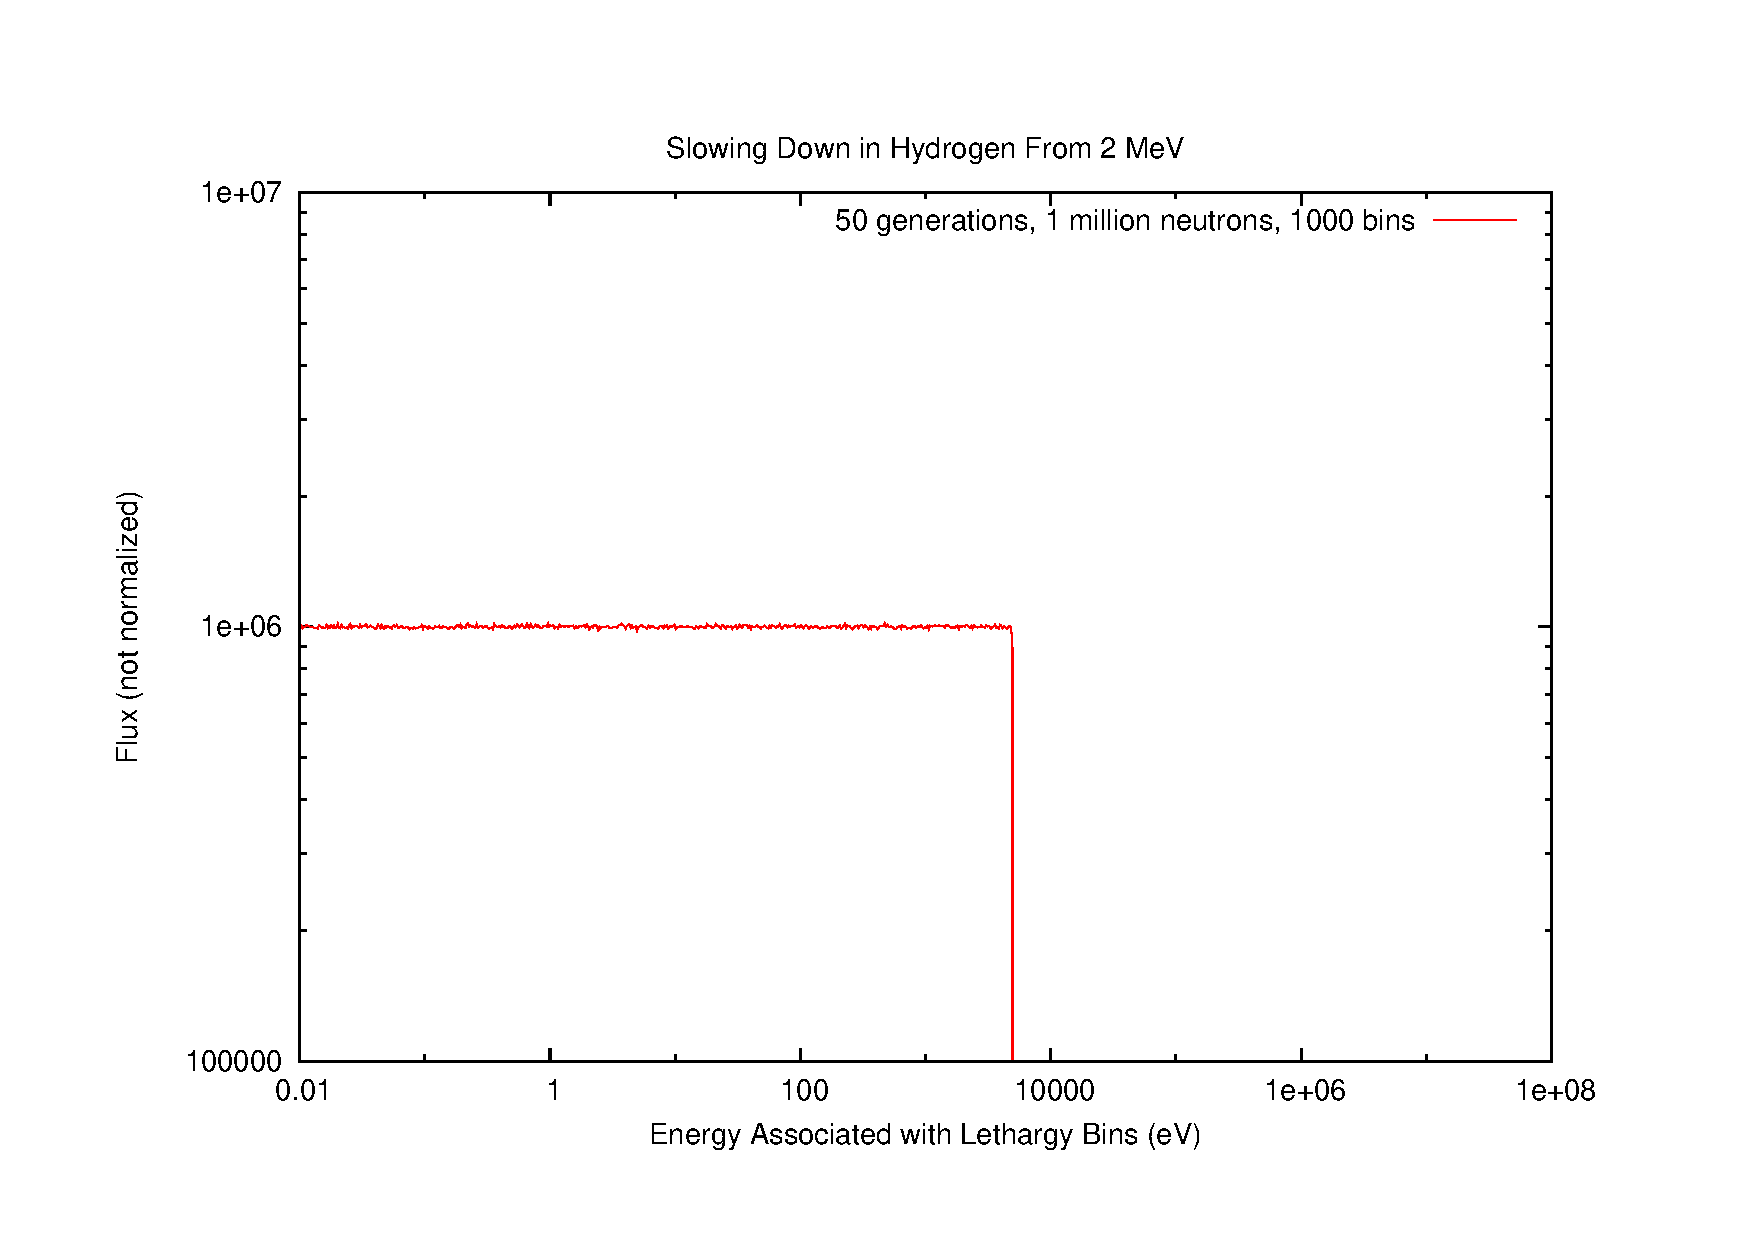
\includegraphics[width=0.3\textwidth]{images/sl-d/spec-1.uncrop.pdf} & asymptotic elastic scattering in hydrogen with source neutrons from 2 MeV \\ 
    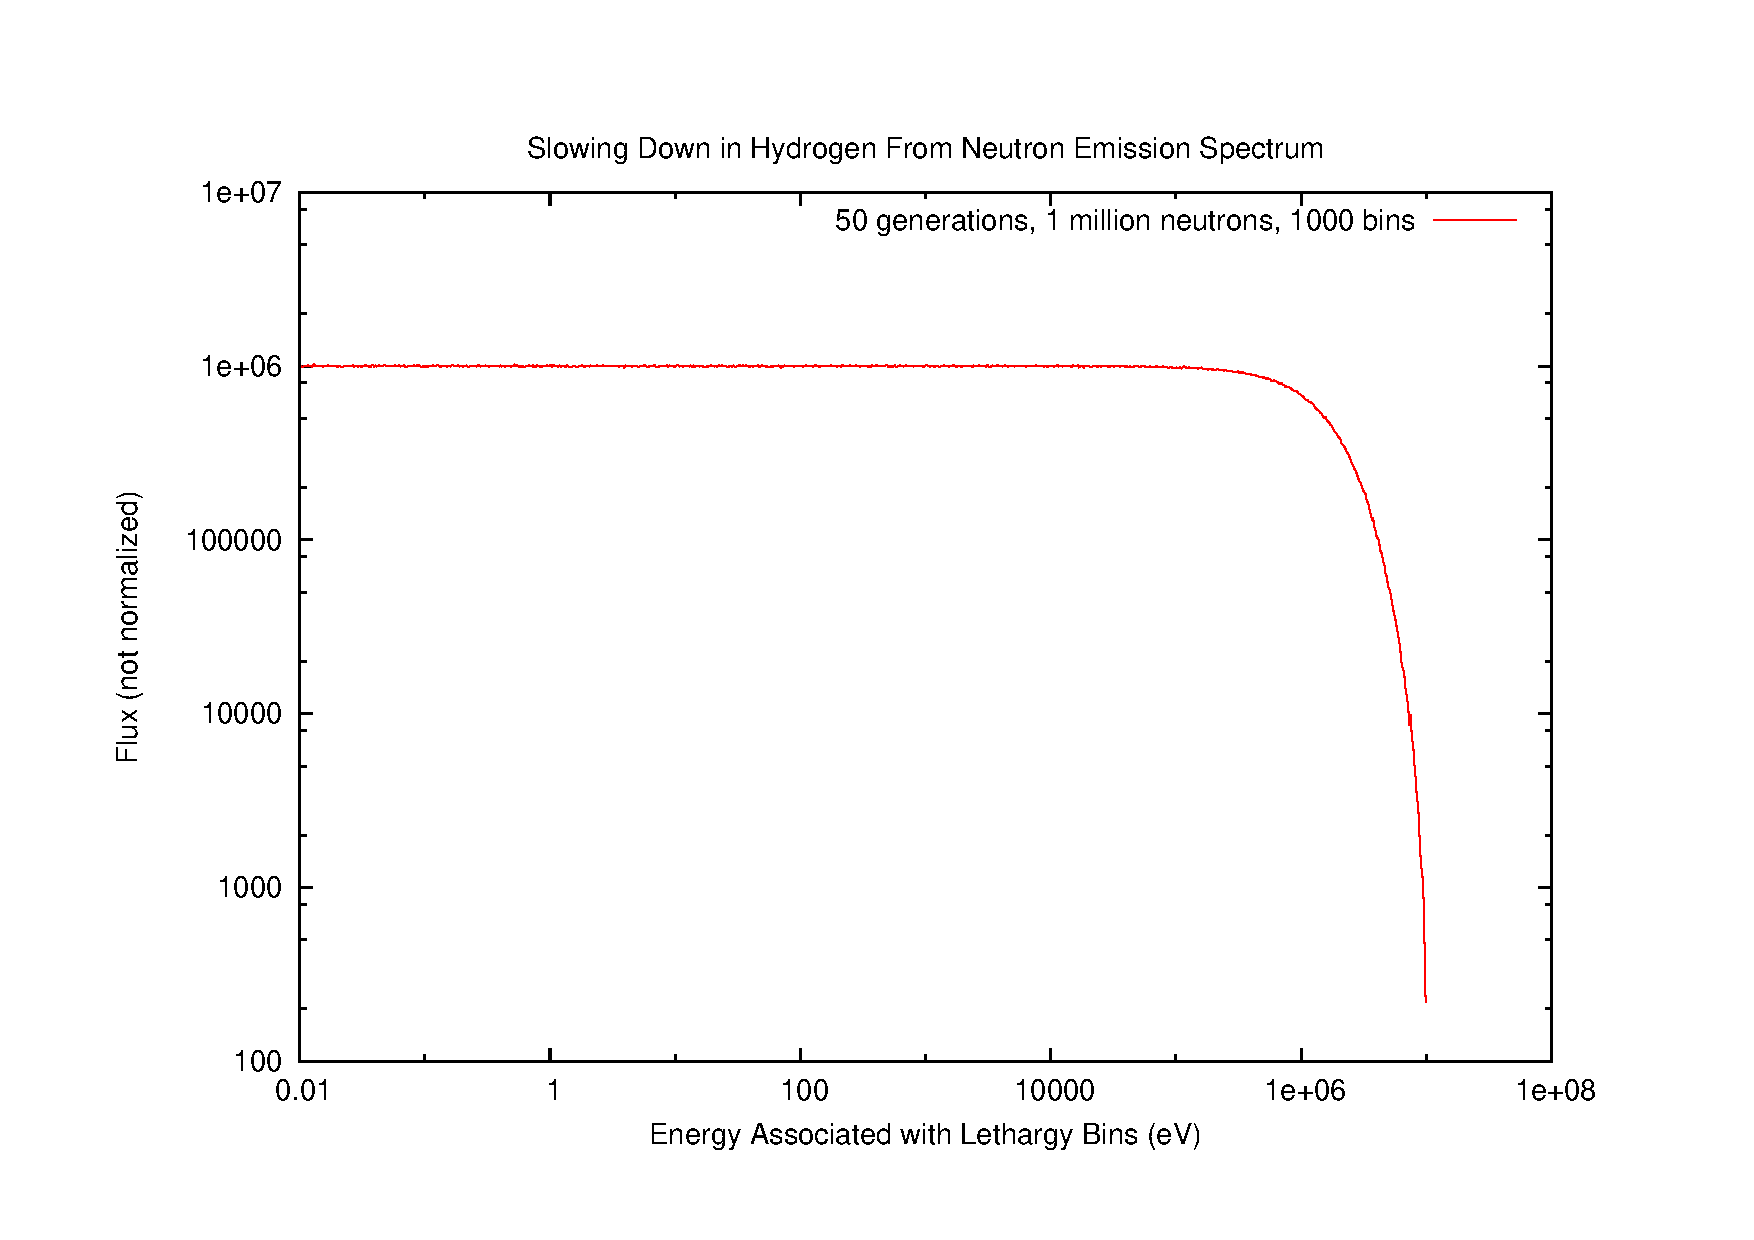
\includegraphics[width=0.3\textwidth]{images/sl-d/spec-2.uncrop.pdf} & replace source neutrons with neutron emission spectrum \\
    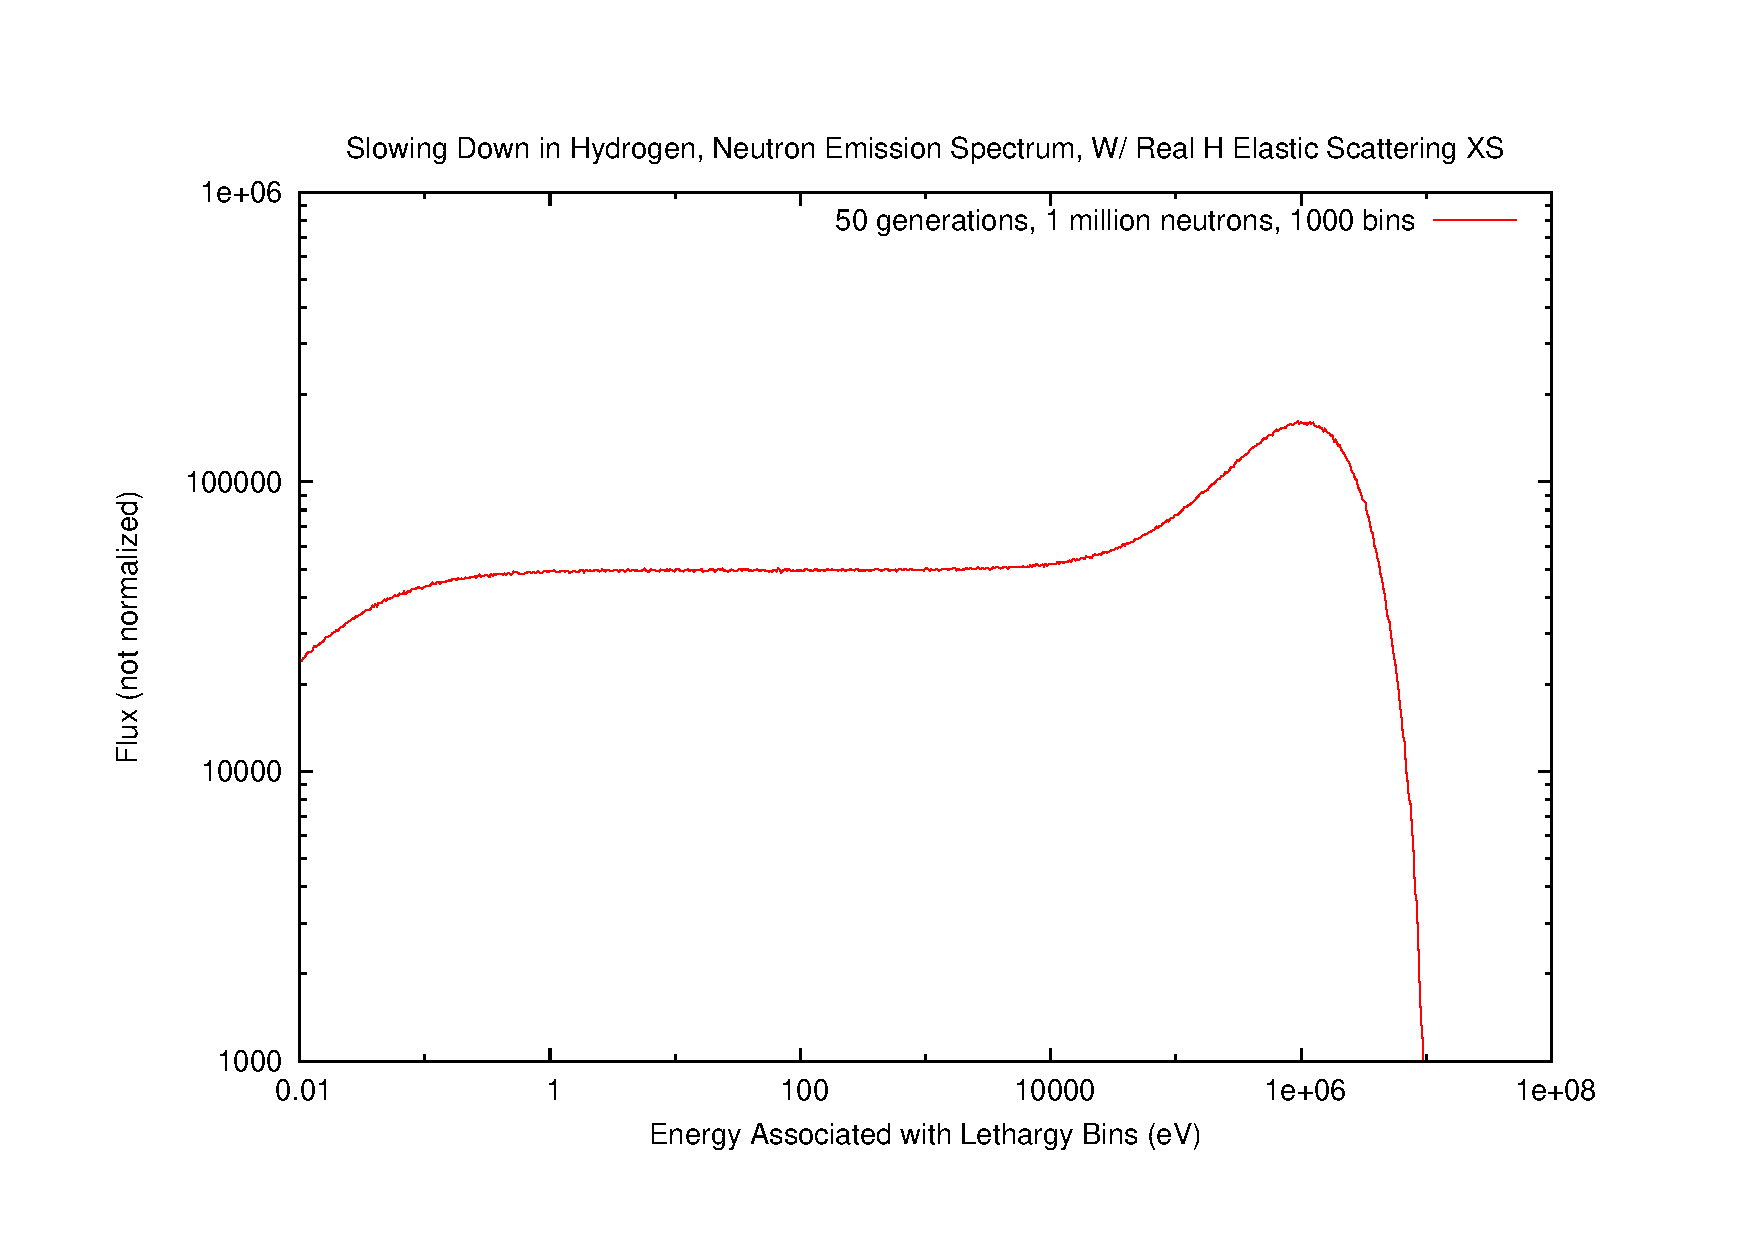
\includegraphics[width=0.3\textwidth]{images/sl-d/spec-3.uncrop.pdf} & add in real H elastic scattering xs (to divide the flux counter by) \\
    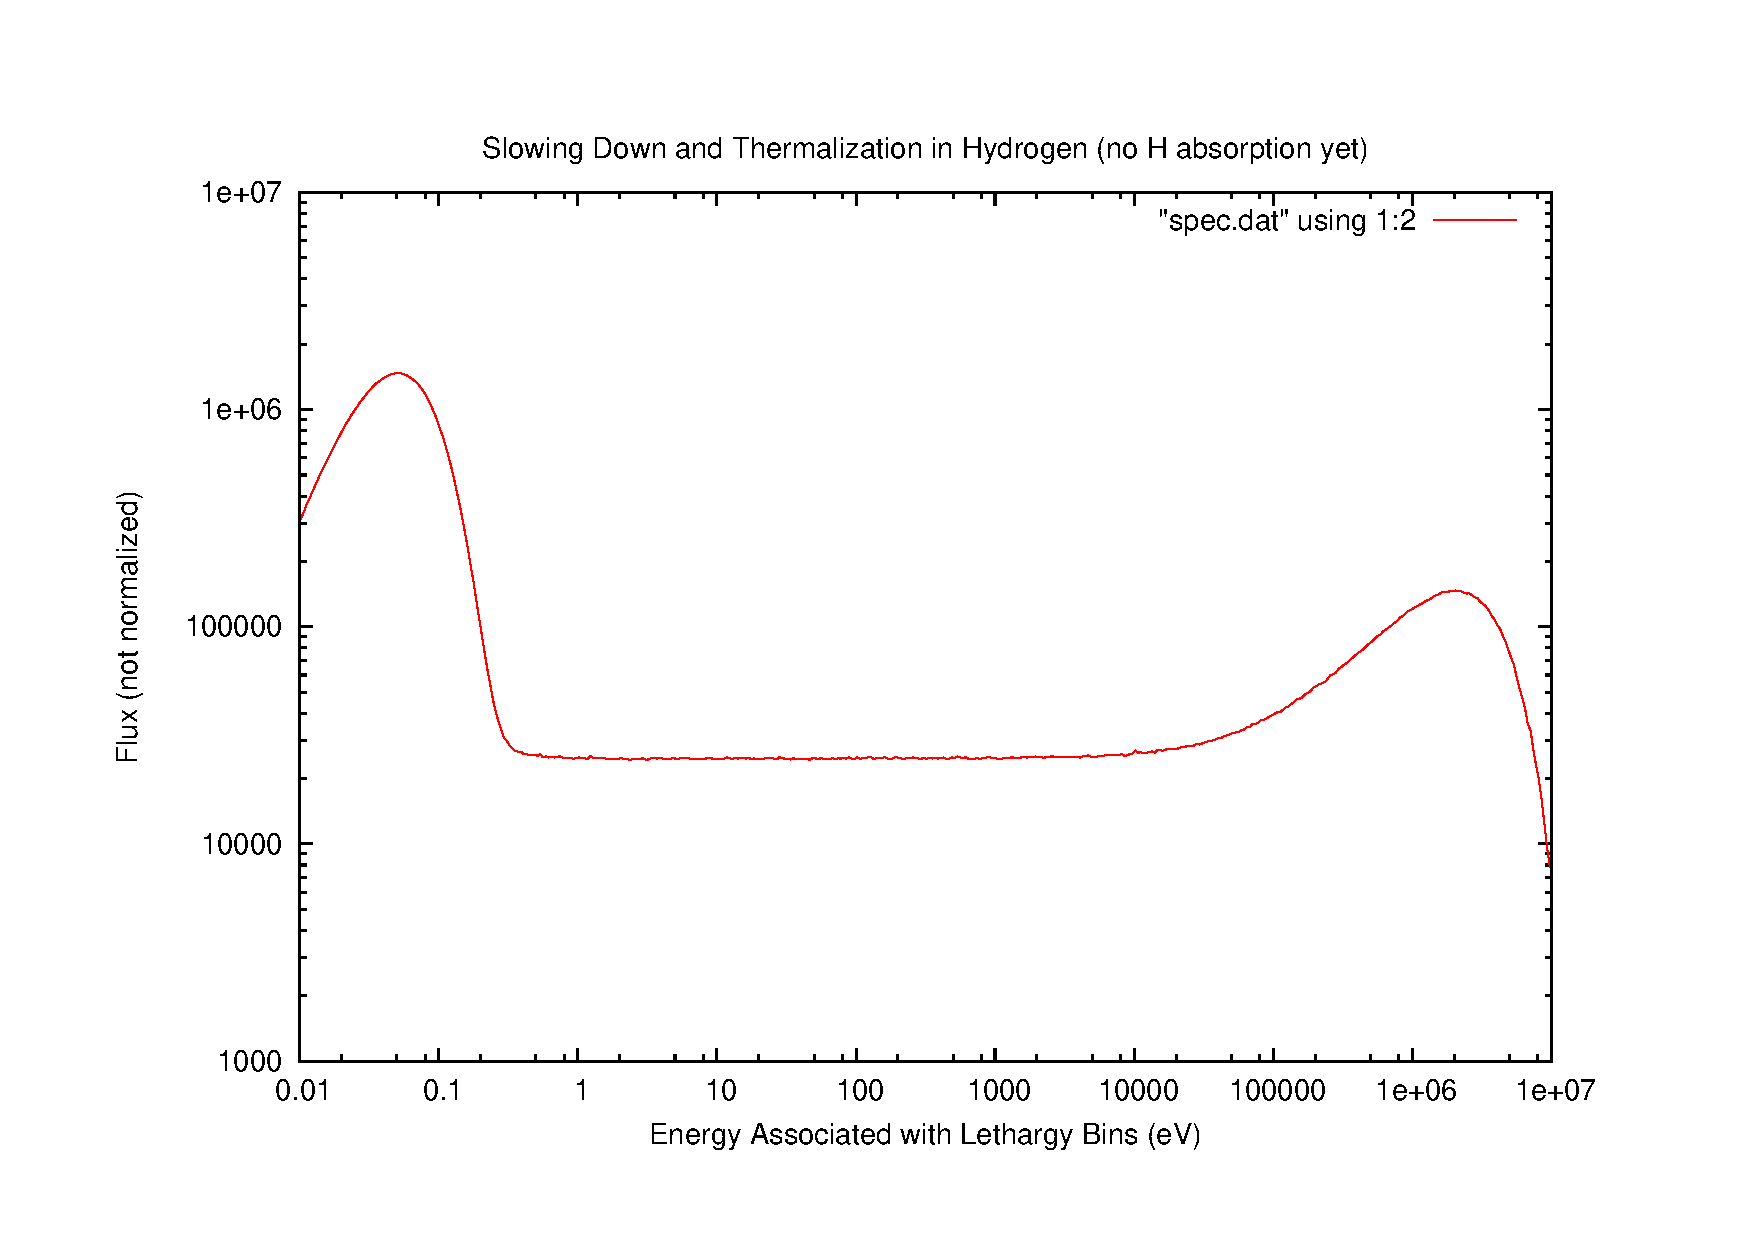
\includegraphics[width=0.3\textwidth]{images/sl-d/spec-4.uncrop.pdf} & add in thermalization in hydrogen ($<$ 4 eV, thermal scattering) \\
    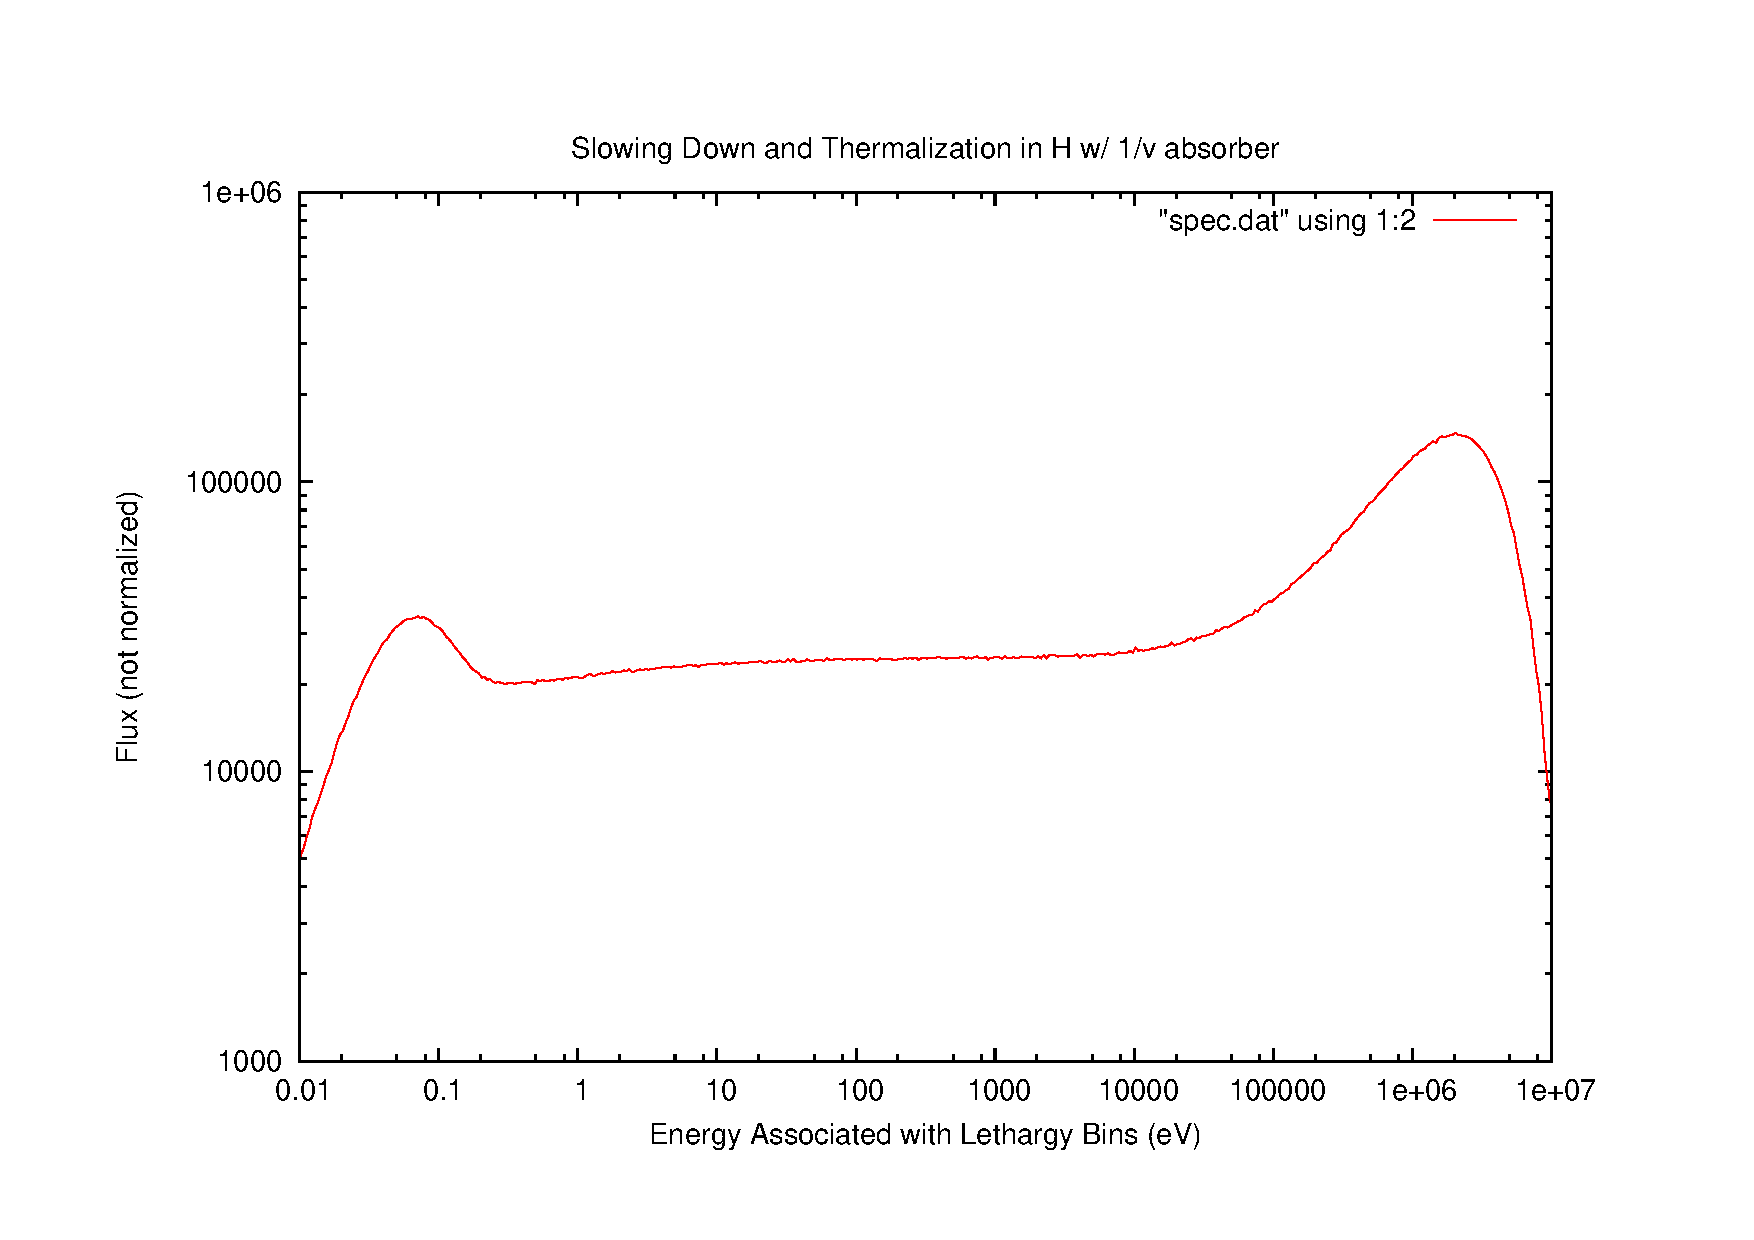
\includegraphics[width=0.3\textwidth]{images/sl-d/spec-5.uncrop.pdf} & add in $1/v$ H absorber (effective only in the thermal range) \\
    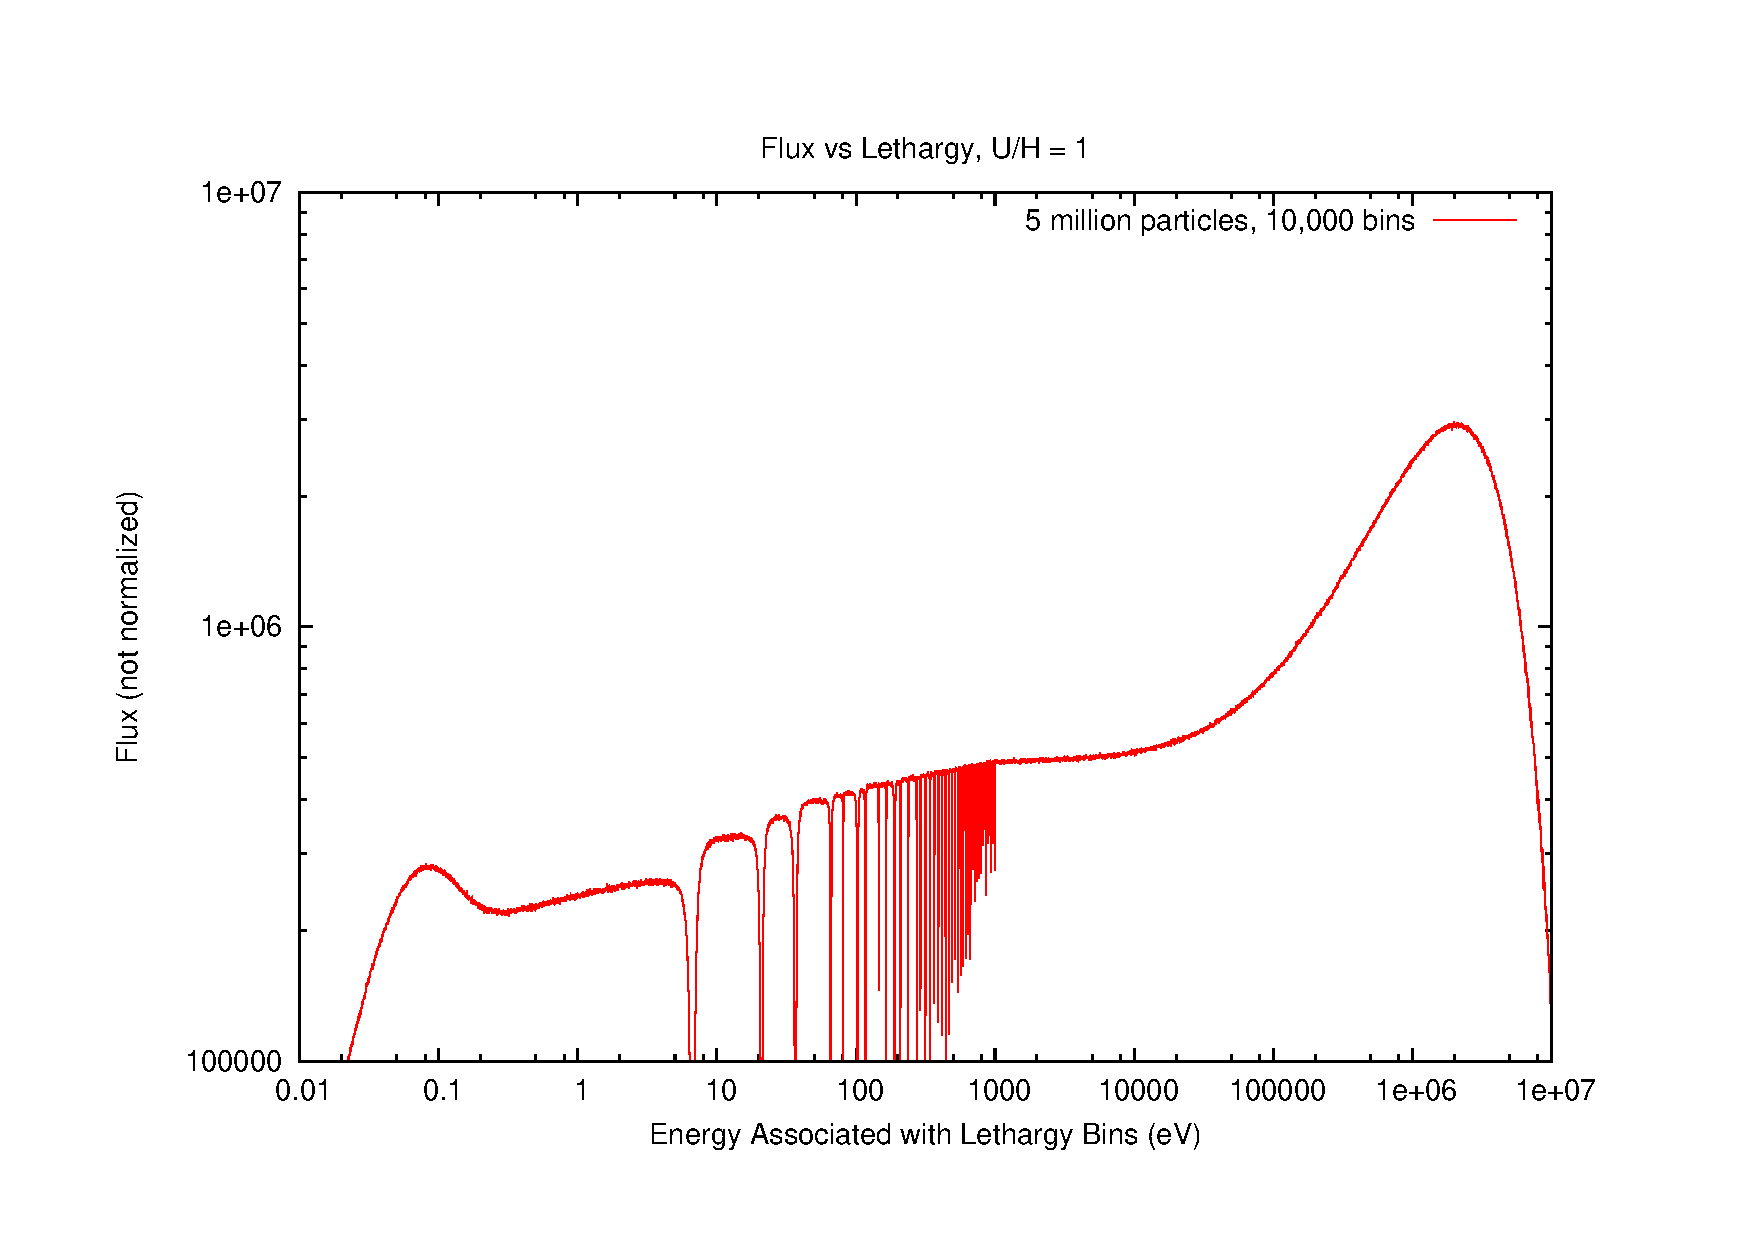
\includegraphics[width=0.3\textwidth]{images/sl-d/spec-7.uncrop.pdf} & add in U238 resonance absorption cross section \\
  \end{tabular}
  \caption{Physics and Their Corresponding Spectra in MC code} \label{plot-MC}
\end{table}
%%%%%%%%%%%%%%%%%%%%%%%%%%%% Exam 1 Review End %%%%%%%%%%%%%%%%%%%%%%%%%%%%%%%%%%%%%%%%%%



\end{document}
